% !TEX root = tesis.tex

\chapter{Detección de partículas energéticas\\ solares con el SciCRT}
\chaptermark{Detección de partículas}
\label{chap:cuatro}
\section{Desempeño del SciCRT como detector de RC}

Estudios sobre el desempeño del SciCRT como detector de rayos cósmicos se encuentran en \cite{ynagai14,ysasai14}, sin embargo hacen la evaluación durante un periodo de tiempo corto y condiciones operacionales distintas a las actuales. En la presente sección enfocaré mis esfuerzos en determinar el desempeño del detector bajo las condiciones actuales de operación, con vistas a determinar su confiabilidad durante un evento de partículas solares y estimar los errores sistemáticos.

Con el fin de alcanzar este objetivo utilicé un código de simulación que incluye las descripción completa del telescopio, el cual fue desarrollado por mi colega Rocío García. Los detalles de esta simulación se presentan en \cite{garcia20}. Algunos puntos que fueron necesarios adaptar para mi análisis son los siguientes:

\begin{itemize}
  \item Considerar siete tipos de partículas diferentes: neutrones, protones, $\mu^{\pm}$, $e^{\pm}$ y rayos $\gamma$.
  \item Utilizar el modelo PARMA como generador de eventos para las distribuciones de energía y de ángulos cenitales.
  \item Los parámetros de entrada del modelo son los correspondientes a la localidad de Sierra Negra y el periodo de observación de Septiembre de \num{2017}.
  \item Todas los espectros de energía de las partículas usadas en la simulación se definen en un rango de \SI{10}{\mega\electronvolt} a \SI{1}{\tera\electronvolt}.
  \item Los propiedades ópticas de los materiales del detector están deshabilitadas para reducir el tiempo de computo.
  \item Se simulan en total \num{3e7} de eventos, los cuales son lanzados al detector desde una esfera de \SI{5}{\metre} de radio.
\end{itemize}

La figura \ref{fig:sim-setup} muestra la geometría usada en la simulación para inyectar las partículas al detector. El cubo azul representa la posición del detector en la simulación, mientras que las partículas son inyectas desde la esfera.

\begin{figure}
        \centering
        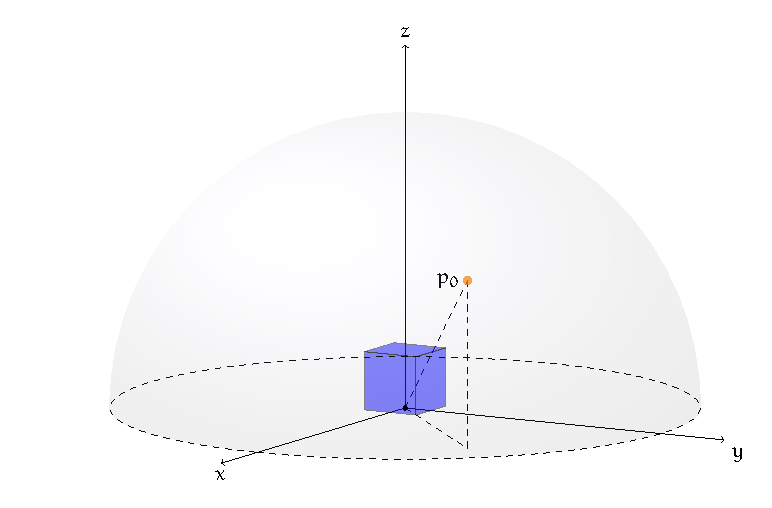
\includegraphics[width=0.75\textwidth]{sim-setup.pdf}
        \caption{Configuración de la simulación en Geant4.}
        \label{fig:sim-setup}
\end{figure}

La condición para que las partículas sean contadas en la simulación es que éstas depositen al menos \SI{7}{\mega\electronvolt} en una barra de cada lado del detector; sin generar señal en las capas dedicadas a la detección de muones. A partir de aquí seleccioné solo los eventos que cumplen con el disparo en el SB \num{3}, que es donde está instalada la electrónica de alta velocidad. El resultado de este análisis se muestra en la figura \ref{fig:total-efficiency}. La línea roja representa la eficiencia de detección de neutrones; mientras que las lineas verde, café, morada, azul y naranja son eficiencias de protones, $\mu^{\pm}$, rayos $\gamma$, positrones y electrones; respectivamente. En todos los casos las eficiencias reportadas son las totales, es decir, están ponderadas con respecto a la distribución angular e incluyen una barra de error. La tasa de eventos total estimada a partir de estas especies es de \SI{3132.31(9480)}{eventos \per\minute}, de los cuales las principales contribuciones provienen de neutrones, muones, rayos $\gamma$ y protones.

Las partículas cargadas son rechazadas de manera eficiente usando la señal de anti-coincidencia, sin embargo éstas puede entrar por los lados del detector. Aun así, dado que electrones, positrones y muones depositan en promedio poca energía por barra (aunque tienen una deposición de energía grande en el detector), el umbral de \SI{7}{\mega\electronvolt} constituye una barrera para estas especies. El caso de los protones es más complejo
puesto que pueden tener deposiciones de energía similares a las de los neutrones.

De acuerdo con este estudio, el SciCRT tiene una eficiencia de detección grande (comparable con la de neutrones) para rayos $\gamma$ con ángulos mayores a \SI{30}{\degree} y energías superiores a \SI{100}{\mega\electronvolt}; lo cual un buen detector de rayos $\gamma$ solares.

\begin{figure}
        \centering
        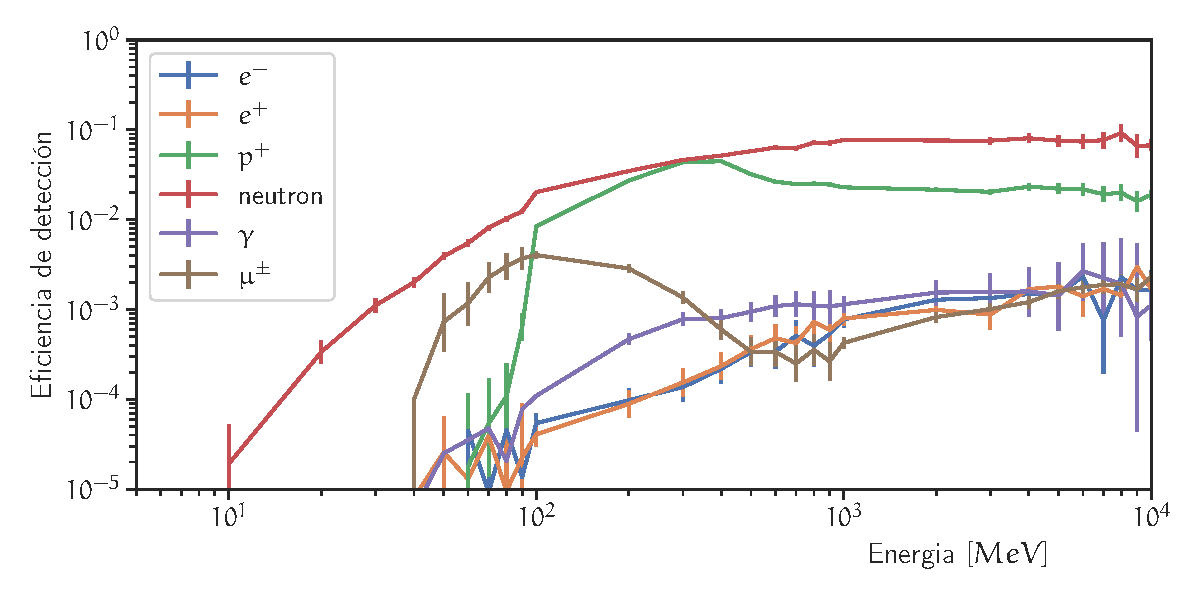
\includegraphics[width=\textwidth]{scibar-efficiency.pdf}
        \caption{Eficiencia de detección del SciCRT para diferentes especies de partículas en función de la energía incidente.}
        \label{fig:total-efficiency}
\end{figure}

El siguiente paso de mi análisis fue comparar la tasa estimada previamente con los datos experimentales. Los datos usados en este parte del análisis provienen del \num{14} de Noviembre de \num{2017}. La tasa de eventos crudos registrada por el telescopio se muestra en la figura \ref{fig:neutron-1pix}. De este modo la tasa media de eventos se estima en: \SI{3841.68(214)}{eventos \per\minute}.

\begin{figure}
        \centering
        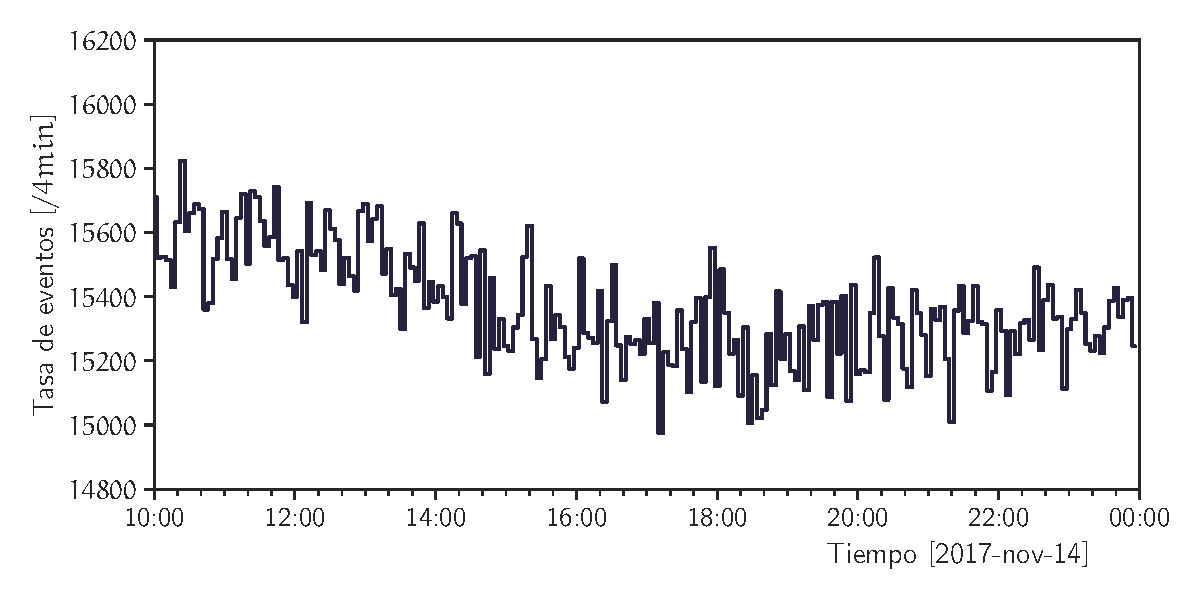
\includegraphics[width=\textwidth]{neutron-171114-1pix.pdf}
        \caption{Tasa de eventos registrada por el SB3 durante el \num{14} de Noviembre de \num{2017}}
        \label{fig:neutron-1pix}
\end{figure}

La diferencia entre la simulación y el experimento es evidente, con un error de \SI{\approx 20}{\percent} tomando como base la simulación. En principio las diferencias deben ser ocasionadas por características del detector no incluidas en la simulación, como pueden ser; las ganancias de los MAPMTs, no linealidades de la electrónica y fluctuaciones debidas a la temperatura, entre otros factores. Dado que las fluctuaciones debidas a la temperatura se deben observar en escalas de tiempo mayores, en primera instancia quedan descartadas como posibles factores que expliquen la discrepancia.

Para poder investigar cualquiera de las posibilidades restantes es necesario reconstruir los eventos registrados por el detector. En resumen este proceso consta de: eliminar el pedestal de las distribuciones de ADC, corregir el efecto de atenuación en las barras y finalmente convertir los valores de ADC en energía depositada.

Una ejemplo de distribución ADC de una de las barras de centelleo se muestra en la figura \ref{fig:neutron-pedestal}. Dos de las características importantes de estas distribuciones son el pico debido a ruido electrónico (pedestal) y el pico de señal (en este caso aproximadamente en \SI{100}{ADC}). Para cada archivo de eventos registrados es necesario estimar el valor del pedestal por barra, ya que éste representa el punto de referencia a partir del cual la electrónica mide la energía depositada. La posición del pedestal de cada barra la calculo a partir de la media de una distribución Gaussiana ajustada al pico principal. La distribución que se muestra en la figura \ref{fig:neutron-pedestal} corresponde a los datos de una barra, acumulados durante una día y a los que se les ha sustraído el pedestal.

\begin{figure}
        \centering
        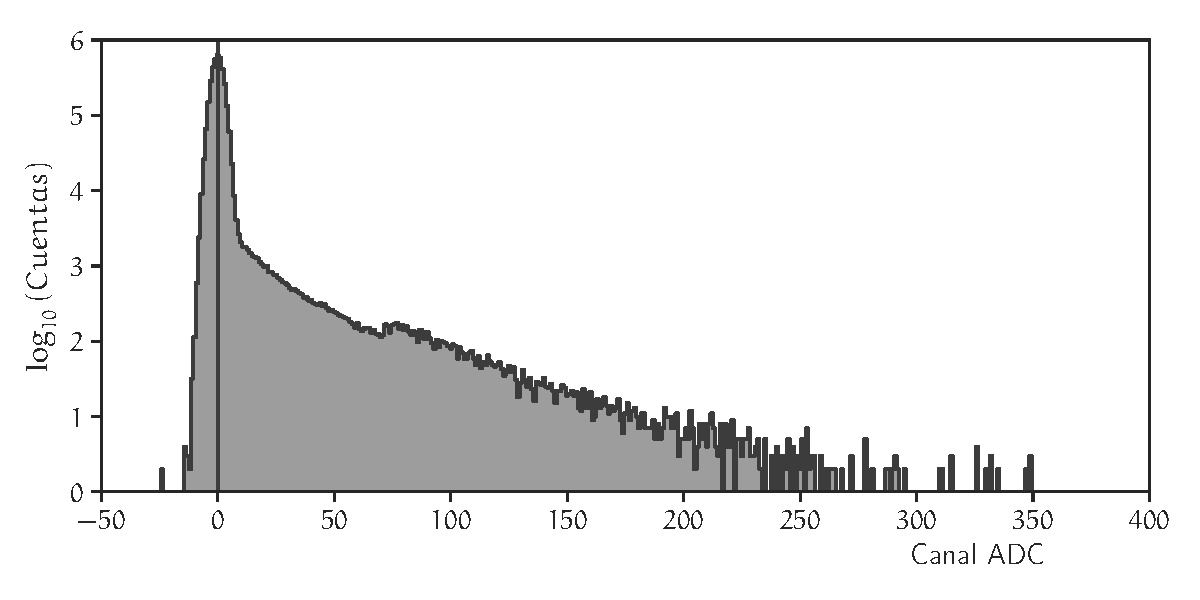
\includegraphics[width=\textwidth]{neutron-ped.pdf}
        \caption{Distribución ADC de una barra de centelleo.}
        \label{fig:neutron-pedestal}
\end{figure}

Posteriormente es necesario corregir los datos de ADC por efectos de la atenuación en la fibra. Este procedimiento se realiza a través de la ecuación \ref{equ:fiber-att}, mencionada previamente. Finalmente los datos de ADC son convertidos a energía depositada usando el mapa de ganancias descrito en \cite{hikimochi16}.

Utilizando los datos de energía depositada, construí distribuciones de energía máxima por traza $E_{max}$, para el periodo de tiempo analizado. El resultado se muestra en la figura \ref{fig:neutron-mindep}, en donde la distribución azul corresponde a las barras del lado Y del SciCRT y la distribución naranja a las del lado X. Estas distribuciones son útiles ya que permiten estudiar el umbral de detección de las barras, y de esta manera nos permiten observar si las diferencias detectadas provienen de la electrónica y/o los MAPMTs. A partir de la figura podemos corroborar que el umbral de detección de las barras es menor a \SI{7}{\mega\electronvolt}, lo cual explica la mayor tasa de eventos en el experimento.

\begin{figure}
        \centering
        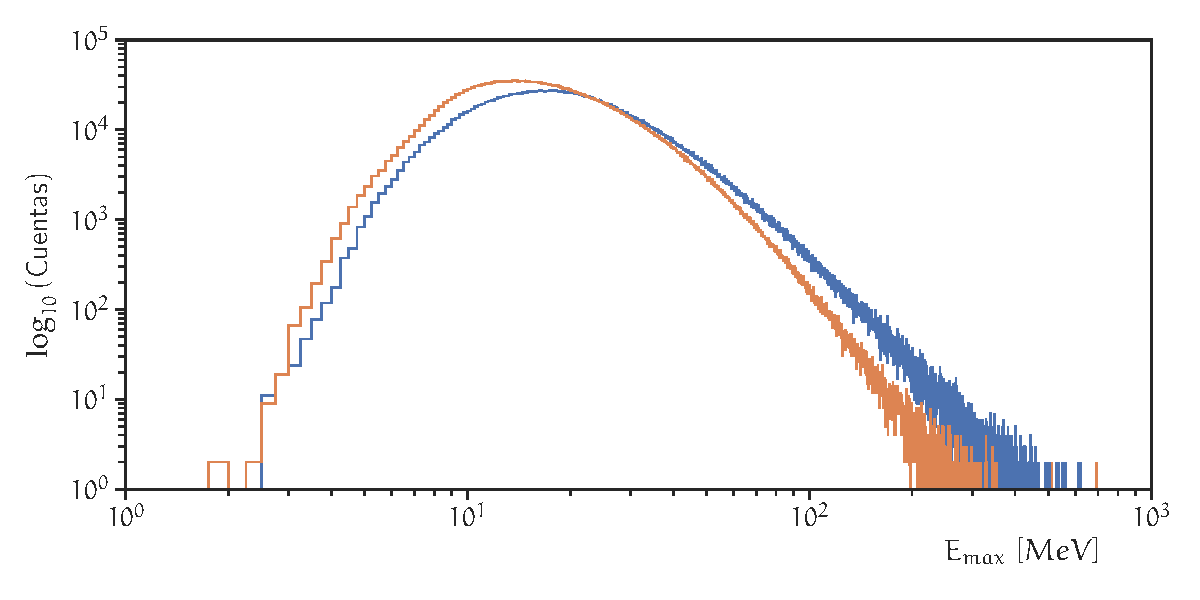
\includegraphics[width=\textwidth]{neutron-mindep.pdf}
        \caption{Distribuciones de energía máxima depositada en una barra de centelleo. La distribución en azul corresponde a las barras del lado Y y la distribución naranja al lado X.}
        \label{fig:neutron-mindep}
\end{figure}

El origen de este fenómeno muy probablemente se debe a unidades de electrónica FE que presentan una ganancia mayor a la del promedio, y por lo tanto permiten registrar eventos de menor energía. La figura \ref{fig:scibar-threshold} permite comprobar este comportamiento. En ella he obtenido las mismas distribuciones de energía máxima depositada, pero en esta ocasión clasificándolas de acuerdo al número de MAPMT donde se detecto el evento. El panel izquierdo muestra en total \num{28} distribuciones, correspondientes a cada uno de los MAPMTs que comprenden el SB3. Se puede apreciar de esta gráfica que la distribución de cada MAPMT inicia en un valor de energía diferente, lo cual apunta a diferencias en el umbral detección. Para observar más claramente este efecto, el panel derecho muestra las distribuciones acumuladas; a partir de las cuales podemos calcular un umbral promedio de \SI{5}{\mega\electronvolt}.

\begin{figure}
        \centering
        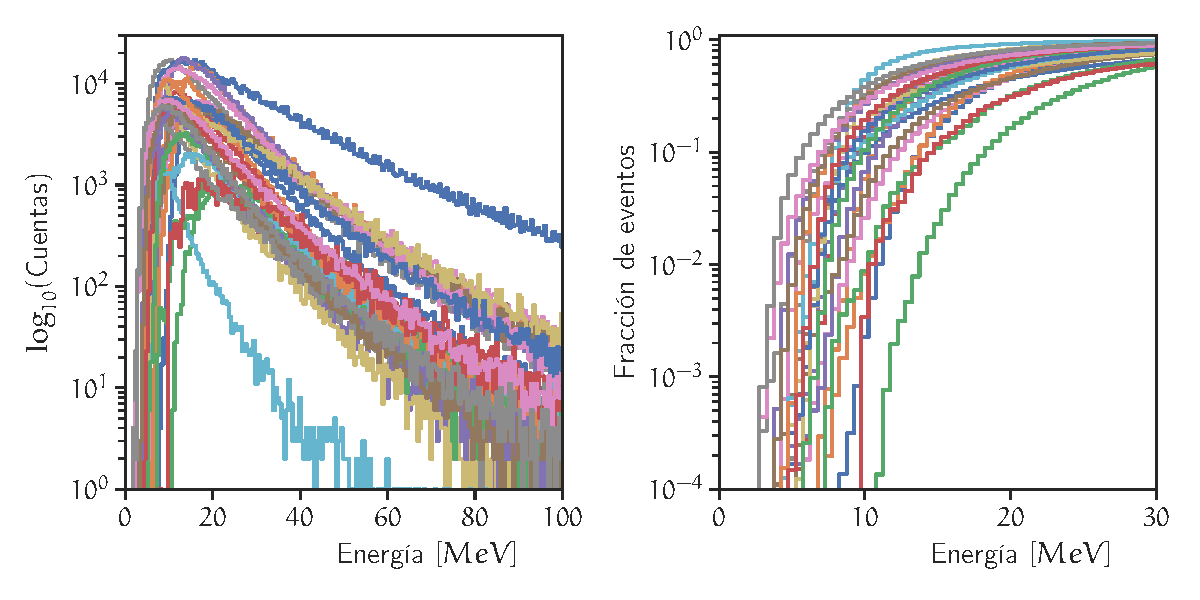
\includegraphics[width=\textwidth]{scibar-threshold.pdf}
        \caption{Distribuciones de energía máxima depositada en una barra de centelleo, clasificadas de acuerdo al MAPMT que registra la señal. El panel izquierdo muestra la distribución de cada fotosensor, mientras que el panel derecho muestra las distribuciones acumuladas.}
        \label{fig:scibar-threshold}
\end{figure}

No obstante, el efecto de este menor umbral solo afecta una pequeña cantidad de eventos; ya que la razón entre el número de eventos que no superan el umbral de \SI{7}{\mega\electronvolt} y los que si solo superan es tan solo del \SI{3.5}{\percent}. Esto podría indicar que el número de canales en la electrónica que permiten el paso de eventos de menor energía es muy pequeño. Luego entonces podemos considerar todos los eventos por debajo de \SI{7}{\mega\electronvolt} como hits accidentales y eliminarlos de nuestro análisis. Finalmente podemos estimar la tasa de eventos del experimento en: \SI{3178.40(177)}{eventos \per\minute}, lo cual concuerda con la simulación dentro de la incertidumbre asociada.

\subsection{Estabilidad del detector}

Para finalizar esta sección presentaré un análisis sobre la operación estable del telescopio. Dado que el SciCRT se encuentra operando en alta montaña, bajo condiciones atmosféricas severas, una parte importante de nuestro trabajo en sitio ha sido el desarrollo e instalación de la infraestructura necesaria. Esto incluye sistemas de respaldo de alimentación eléctrica (banco de baterías y fuente de alimentación ininterrumpida) y sistema de ventilación para favorecer la disipación de calor de la electrónica. La figura \ref{fig:muon-monthly} presenta un ejemplo de la operación estable del detector durante el mes de febrero de \num{2020}. En esta figura se muestran los datos del número de eventos por hora registrados en las capas de muones en color azul oscuro, mientras que la linea azul claro presenta los datos del NM de la Ciudad de México. A fin de presentar ambas gráficas en la misma escala, sume \SI{e6} cuentas a los datos del NM. De la gráfica se puede observar que ambas series de tiempo siguen la misma evolución en el tiempo, lo cual es notable para en el caso de un detector operando a la altura de Sierra Negra ya que los NMs son instrumentos ampliamente usados en el estudio de RC debido a su estabilidad.

\begin{figure}
        \centering
        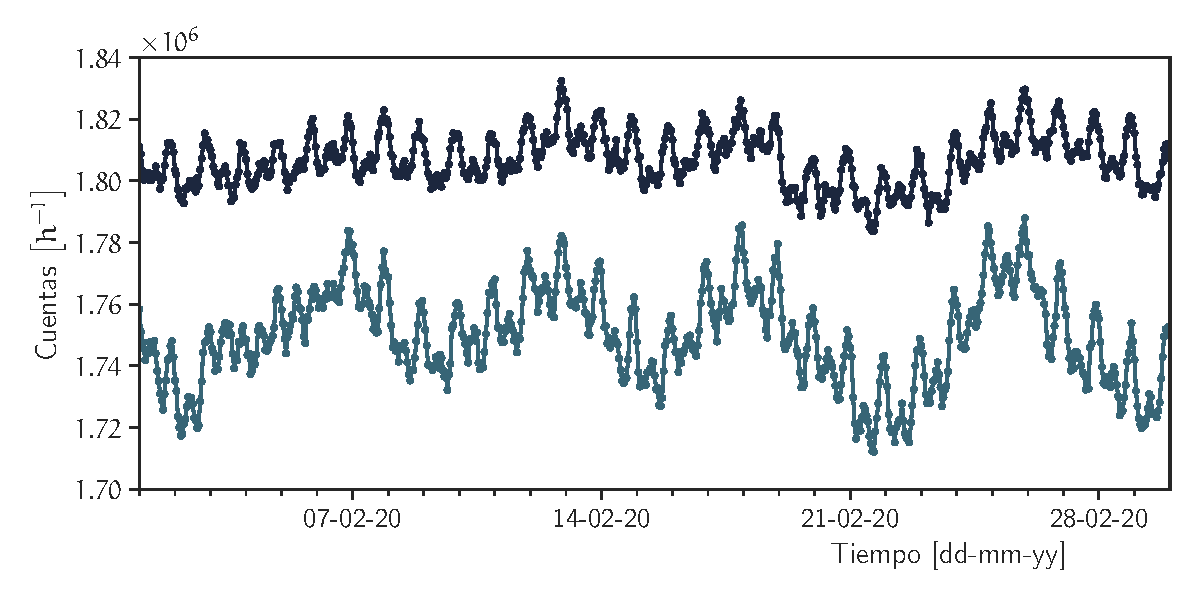
\includegraphics[width=\textwidth]{muon-monthly.pdf}
        \caption{Total de eventos de muones registrados durante Febrero \num{2020} por el SciCRT (linea azul oscura) en comparación con datos del NM de la Ciudad de México (línea azul claro).}
        \label{fig:muon-monthly}
\end{figure}

De forma simular la figura \ref{fig:neutron-monthly} muestra el número de eventos por hora de las capas de neutrones. En este punto es importante aclarar que, debido al gran volumen de datos que registra el SB3, la adquisición en esta capa del detector se detiene por las noches para poder comprimir los archivos registrados. Esto explica las discontinuidades que se observan en la gráfica. A pesar de esta limitante, se pueden notar de la figura que la serie de tiempo sigue la misma tendencia de las otras mencionadas previamente.

\begin{figure}
        \centering
        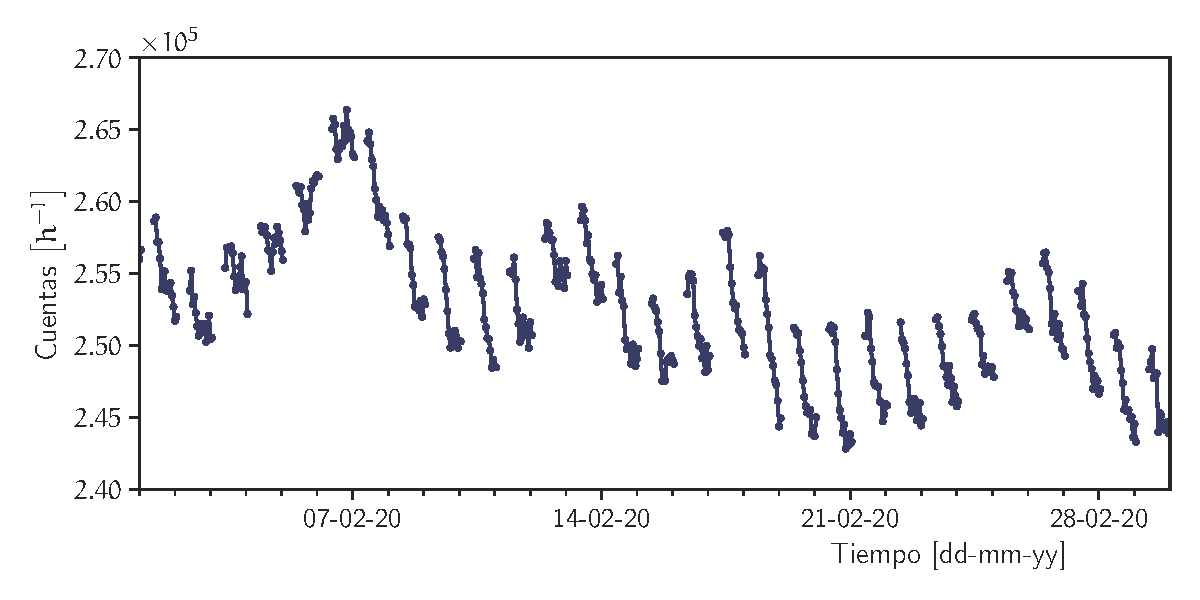
\includegraphics[width=\textwidth]{neutron-monthly.pdf}
        \caption{Total de eventos de partículas neutras registrados durante Febrero \num{2020} por el SciCRT.}
        \label{fig:neutron-monthly}
\end{figure}

Por otra parte, ya que una parte significativa del análisis con los datos de neutrones está relacionada con la deposición de energía en las barras, un estudio de estabilidad requiere monitorear las ganancia de los MAPMTs en función del tiempo. La figura \ref{fig:mip-stability} muestra el resultado de esta análisis para los MAPMTs en las capas de neutrones, durante un periodo de tres; de Diciembre \num{2019} a Febrero \num{2020}. Para calcular la ganancia de los MAPMTs, dado que el pico de señal no es muy prominente, el procedimiento análisis es el siguiente:

\begin{enumerate}
  \item Usando las distribuciones de ADC de cada barra y calcular los pedestales (ver figura \ref{fig:neutron-pedestal}).
  \item Ajustar una función exponencial negativa a la región de \num{15} a \SI{70}{ADC} posterior al pico del pedestal.
  \item Sustraer el pedestal y función exponencial de la distribución de la barra.
  \item Estimar la posición del pico de la señal.
\end{enumerate}

El paso final se puede realizar ajustando una distribución al histograma resultado o calculando la moda del mismo. Por simplicidad del algoritmo utilicé la moda del histograma, sin embargo, resultados similares se pueden obtener ajustando una distribución. La desventaja de usar la moda es que este es parámetro muy sensible a la estadística del histograma, lo cual contrarreste calculando la ganancia en periodos de tres días. El panel superior de la figura \ref{fig:mip-stability} muestra la variación de la ganancia en el tiempo para uno de los MAPMTs del SB3. Como se observa en la figura, la ganancia tiene fluctuaciones considerables durante el periodo, muy probablemente causadas por efectos de temperatura \cite{knitta04}. No obstante, la mayoría de las variaciones están en el intervalo del \SI{\pm 1.0}{\percent} (área sombreada en verde oscuro) y ninguna sobrepasa \SI{\pm 2.0}{\percent} (área sombreada en verde claro).

Finalmente el panel inferior muestra la distribución para todo los MAPMTs en el SB3 durante el periodo de tres meses. De la figura se puede concluir que, a pesar de las condiciones atmosféricas de Sierra Negra, todas las variaciones se encuentran en el rango de \SI{\pm 2.5}{\percent}.

\begin{figure}
        \centering
        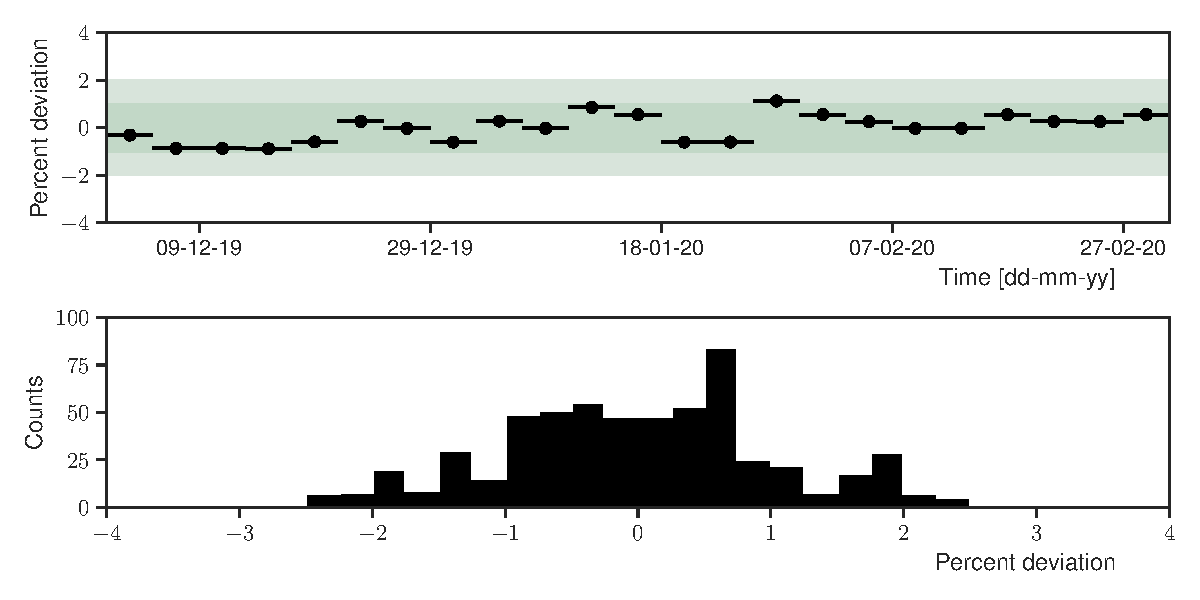
\includegraphics[width=\textwidth]{neutron-mip_stability.pdf}
        \caption{Estabilidad de la ganancia de los MAPMTs durante un periodo de tres meses. El panel superior muestra la variación en el tiempo de uno de los MAPMT. Las áreas sombreadas corresponden con las variaciones de \SI{\pm 1}{\percent} y \SI{\pm 2}{\percent}. El panel inferior es la distribución de todos los MAPMTs.}
        \label{fig:mip-stability}
\end{figure}

\section{Observación de partículas solares}

Una vez demostrada la operación estable del SciCRT, así como las posibles fuentes de error asociadas con la electrónica; en lo que resta de este capitulo mostraré las capacidades del telescopio en la observación de partículas energéticas solares. Para lograr este objetivo, mi análisis complementa las observaciones hechas con el SciCRT con datos obtenidos mediante satélites dedicados a la detección de rayos X y $\gamma$. Las misiones satelitales utilizadas en este estudio son: FERMI, RHESSI, y GOES \num{15}.

Los datos de GOES \num{15} (obtenidos de \cite{goesdata}) sirven como punto de partida para el estudio, ya que este satélite lleva un registro las \SI{24}{\hour} del flujo de rayos X provenientes del Sol. De acuerdo con la tabla \ref{table:eventos-neutrones} la mayoría de los eventos de neutrones solares están asociados con ráfagas del tipo X, mientras que solo un evento está confirmado se produjo por una ráfaga tipo M. Considerando la base de datos de GOES, desde la instalación de la electrónica de alta velocidad en el SciCRT (Julio \num{2015}) a la fecha; se han detectado \num{4} explosiones del tipo X y \num{71} del tipo M.

De los \num{4} eventos más intensos (todos ocurridos en Septiembre de \num{2017}), dos de ellos no coinciden en tiempo con el periodo de observación del telescopio, mientras que en los otros dos el SciCRT no estaba trabajando debido a problemas en el suministro eléctrico del sitio.

Tomando en cuenta que el SciCRT es más sensible a neutrones de baja energía y la intensidad en rayos X está relacionada con el espectro de los neutrones producidos\footnote{Lo cual es una suposición razonable pero aún requiere de más pruebas para sustentarla.}, un estudio sistemático de las \num{71} fulguraciones del tipo M resulta de gran interés para la comunidad, aun considerando que solo una fracción de éstas tiene condiciones para ser detectada en Sierra Negra. No obstante, por restricciones de tiempo solo concentraré mi análisis en dos eventos interesantes ocurridos durante Septiembre de \num{2017}.

\subsection{Posible observación de neutrones solares el 4 de Septiembre de 2017}

El \num{4} de Septiembre de \num{2017} la región activa \num{12673} produjo una fulguración del tipo M\num{5.5} a las \DTMtime{20:28:00} UT (instante en que se registro en la orbita de la Tierra), localizada  en las coordenadas S\SI{10}{\degree} W\SI{02}{\degree} (figura \ref{fig:september-04-flare}). A esta hora el satélite GOES registro un incremento en rayos X suaves en la banda de \num{1.5} a \SI{12}{\kilo\electronvolt}, lo cual se muestra en color negro en la figura \ref{fig:september-04-xrays}.

\begin{figure}
        \centering
        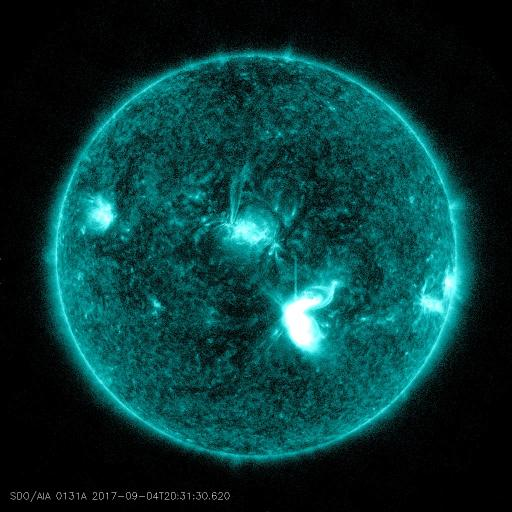
\includegraphics[width=0.7\textwidth]{sdo170904-2030-13}
        \caption{Image tomada por el satélite SDO durante la fulguración del $04/09/17$ en la banda de \SI{13.1}{\nano\metre}. Fuente: \url{https://www.spaceweatherlive.com/en.html}}
        \label{fig:september-04-flare}
\end{figure}

Por otro, la línea verde en la figura \ref{fig:september-04-xrays} muestra los datos del monitor de estallidos de rayos $\gamma$ de FERMI (GBM) en la banda de \num{50} a \SI{300}{\kilo\electronvolt}. Dos incrementos importantes en esta banda se observan a las \DTMtime{20:28:00} y \DTMtime{20:52:00}, lo cual brinda pruebas de la aceleración de electrones durante la explosión. Un análisis similar usando los datos de RHESSI \cite{rhessidata} nos proporciona información similar a la obtenida con FERMI\footnote{No incluyo los datos de RHESSI en este trabajo debido a que no existen herramientas libres para su procesamiento. Sin embargo, un análisis preliminar de éstos se puede hacer en la siguiente página \url{http://sprg.ssl.berkeley.edu/~tohban/browser/}.}.

Para poder argumentar sobre la producción de neutrones durante la ráfaga es necesario buscar en el espectro de rayos $\gamma$ las firmas de los procesos de desexcitación nuclear y decaimiento de piones. No obstante, en este evento en particular, el telescopio de neutrones SEDA-FIB (instalado en la estación internacional) reporta una detección de neutrones en la dirección solar con alta significancia estadística \cite{kamiya19}. Además de esto GOES también reporta un incremento debido a protones de altas energías, observado \SI{4}{\hour} después de la explosión. De esta manera podemos esperar la observación de neutrones en la superficie terrestre si las condiciones de profundidad atmosféricas y flujo son adecuadas.

\begin{figure}
        \centering
        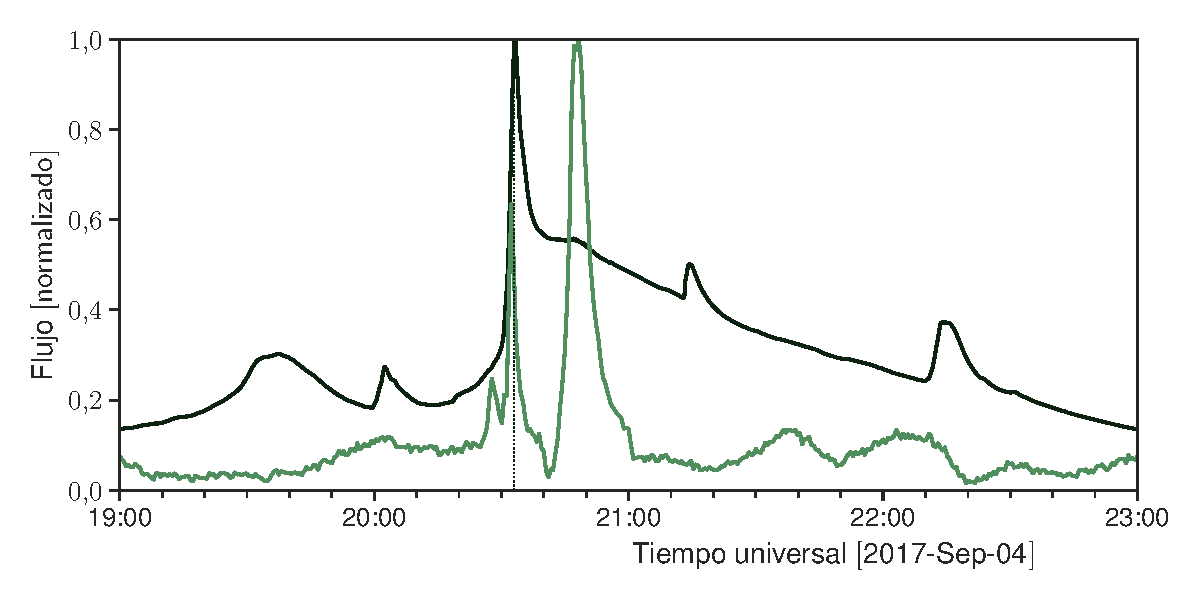
\includegraphics[width=\textwidth]{xrays_170904.pdf}
        \caption{Perfil temporal de rayos X suaves (linea negra) observados por GOES 15, para la fulguración del \num{4} de Septiembre de \num{2017}. La linea verde muestra los datos de FERMI-GBM en el rango de \num{50} a \SI{300}{\kilo\electronvolt}.}
        \label{fig:september-04-xrays}
\end{figure}

La figura \ref{fig:september-04-zenith} muestra el coseno del ángulo cenital solar para las diferentes localidades donde se encuentra la red mundial de telescopios de neutrones, considerando el instante en que se registra el máximo de la ráfaga. A partir de esta figura podemos concluir que en el instante del evento solar las mejores estaciones para observar neutrones solares eran Mauna Kea (Hawaii) y Sierra Negra, México. Tomando en cuenta el caso de México, el valor del ángulo cenital para el momento de la ráfaga es de \SI{38.7}{\degree} y la masa de aire en el sitio \SI{732}{\gram\per\square\cm}. Sin embargo, debido a que los neutrones sufren dispersión elástica en la atmósfera, la masa de aire efectiva es menor (\SI{\approx 650}{\gram\per\square\cm}); lo cual favorece la propagación \cite{dorman99,shibata94}.

\begin{figure}
        \centering
        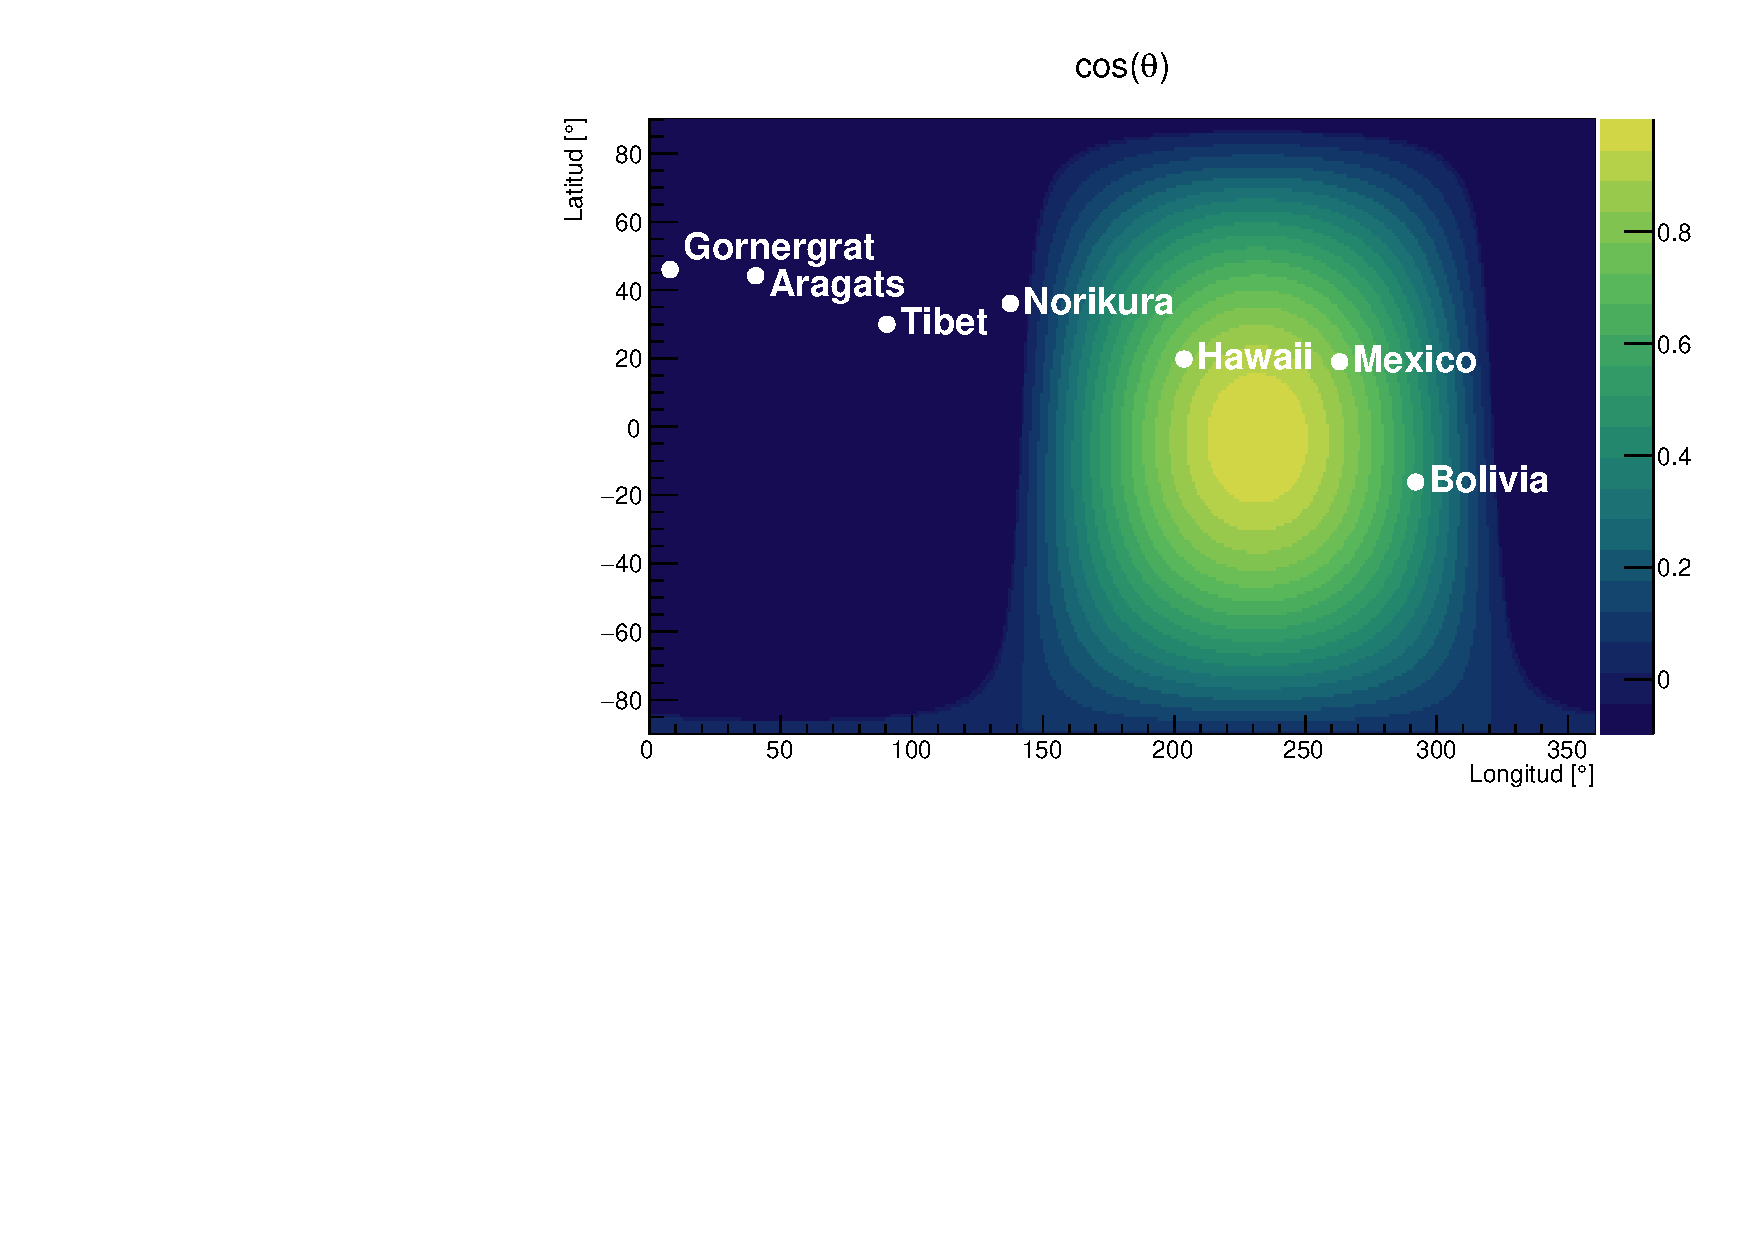
\includegraphics[width=0.8\textwidth]{cosz_170904.pdf}
        \caption{Coseno del ángulo cenital del Sol para el instante en que se registra la ráfaga. Los puntos muestran la localización geográfica de los TNS. La zona más clara indica un ángulo cenital del Sol cercano a cero.}
        \label{fig:september-04-zenith}
\end{figure}

A pesar de que estas condiciones favorecen la observación de partículas solares en Sierra Negra, como se puede apreciar en la figura \ref{fig:september-04-neutrons}, la tasa de eventos del telescopio no registra ningún exceso positivo durante la explosión. En la figura, el instante del máximo de la ráfaga $t_{0}$ se indica mediante la linea punteada vertical. Para calcular la significancia ($\sigma$) de los datos lo hice siguiendo el procedimiento descrito en \cite{diegophd}. En este método, primero ajustamos un polinomio de tercer grado a la serie de tiempo de las cuentas, considerando una ventana de tiempo $t_{0}\pm\SI{1.5}{\hour}$. Posteriormente calculamos la significancia mediante la siguiente expresión:

\begin{equation}
\sigma=\frac{N_{j}-N_{bj}}{\alpha\sqrt{N_{bj}}}
\end{equation}

de donde $N_{j}$ es el total de cuentas registradas por cada \SI{2}{\minute}, $N_{bj}$ es el valor de la linea de base (polinomio) y $\alpha$ un factor de normalización, el cual sirve para \emph{estandarizar} los residuos ($N_{j}-N_{bj}$). A partir de esta expresión consideramos como señal significativa a cualquier exceso de cuentas arriba de $3\sigma$. Para poder asociar esta señal con la detección de partículas solares, es necesario que ésta ocurra dentro del intervalo de tiempo de $t_{0}-\SI{15}{\minute}$ a $t_{0}+\SI{45}{\minute}$; lo cual tiene como objetivo buscar señales de neutrones solares en un amplio rango de energías.

En la figura \ref{fig:september-04-neutrons} la linea azul representa el ajuste del polinomio de tercer grado, mientras que el área sombreada en la dirección horizontal es el intervalo de $\pm 3\sigma$. Como se puede observar, no existe ningún incremento mayor a $3\sigma$ en el área sombreada vertical, en primera instancia no podemos concluir que el SciCRT detector partículas solares.

Por otro lado, dado que la fulguración no es gran magnitud, es conveniente buscar un método para eliminar la contaminación producida por radiación cósmica secundaria en los eventos registrados, y analizar si de esta forma es posible encontrar una señal significativa.

\begin{figure}
        \centering
        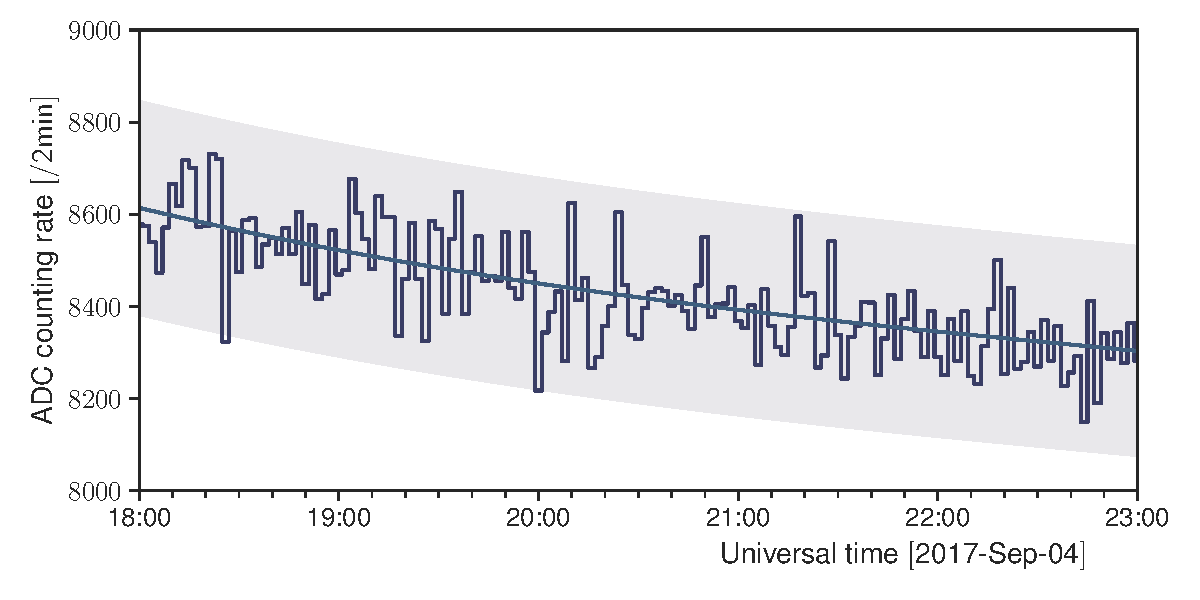
\includegraphics[width=\textwidth]{neutron-170904.pdf}
        \caption{Perfil temporal de eventos registrados por el SciCRT el $04/09/17$. El área sombreada representa el nivel de $3.0\sigma$.}
        \label{fig:september-04-neutrons}
\end{figure}

Un método simple para realizar la clasificación consiste en el análisis de las distribuciones de energía depositada contra energía máxima depositada en una barra \cite{nagaiphd,sasaiphd}. La figura \ref{fig:scicrt-edep-emax} muestra las distribuciones obtenidas mediante simulación para las diferentes componentes de la radiación cósmica. El panel superior muestra los resultados para $e^{\pm}$ y rayos $\gamma$, el panel del centro contiene datos de $\mu^{\pm}$ y el panel inferior corresponde a la componente hadrónica. En todas las figuras la escala de color (de colores claros a oscuros) representa la densidad de eventos en uno de los \emph{bines}. Se puede apreciar en las figuras que tanto las componente electromagnética como la muónica se agrupan en el extremo inferior derecho de las gráficas, mientras que los hadrones están agrupados en la parte superior izquierda. Esto se debe a que los protones tienen pérdidas de energía grandes cuando se detienen dentro del detector.

\begin{figure}
        \centering
        \begin{subfigure}[b]{\textwidth}
                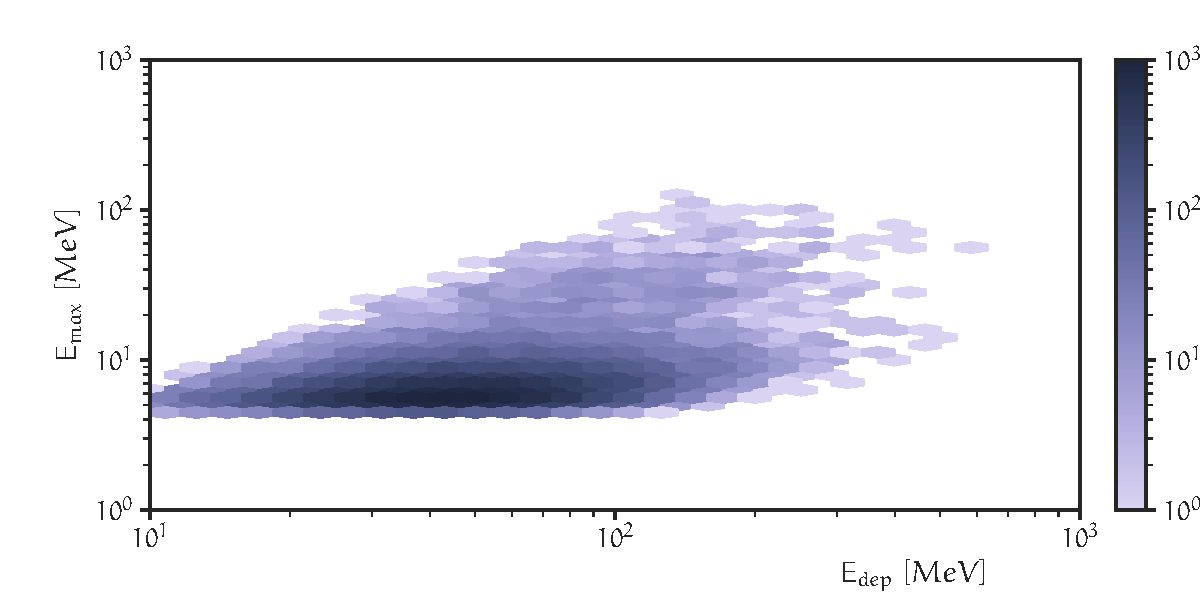
\includegraphics[width=0.725\textwidth]{scibar-em.pdf}
                \caption*{Componente electromagnética ($\gamma$ y $e^{\pm}$).}
        \end{subfigure}
        \begin{subfigure}[b]{\textwidth}
                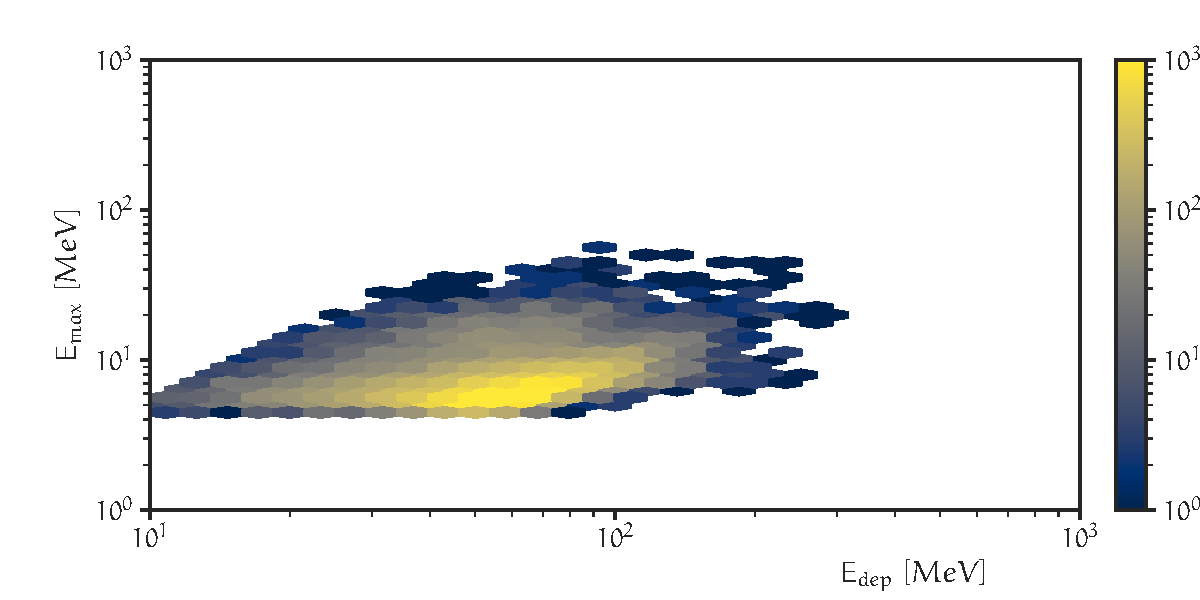
\includegraphics[width=0.725\textwidth]{scibar-mu.pdf}
                \caption*{Componente muónica.}
        \end{subfigure}
        \begin{subfigure}[b]{\textwidth}
                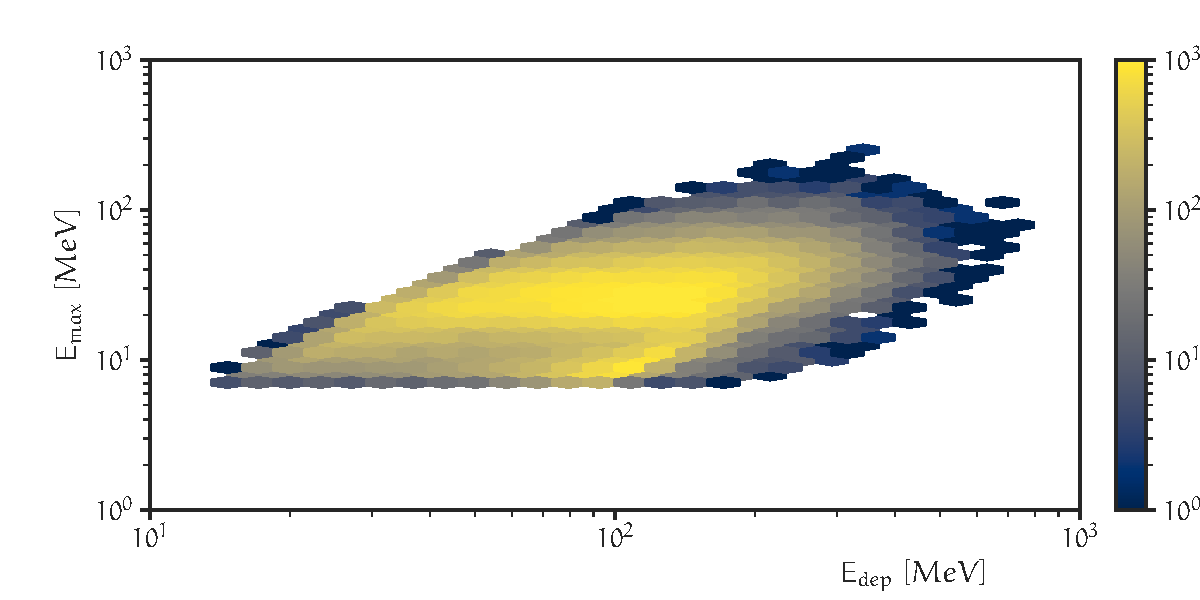
\includegraphics[width=0.725\textwidth]{scibar-had.pdf}
                \caption*{Componente hadrónica.}
        \end{subfigure}
        \caption{Distribuciones $E_{dep}$  $E_{max}$ para las diferentes componentes de la radiación cósmica secundaria.}
        \label{fig:scicrt-edep-emax}
\end{figure}

De esta forma podemos definir la ecuación \ref{equ:edep-disc}, la cual permite realizar la separación entre hadrones y componentes muónica/electromagnética:

\begin{align}
\label{equ:edep-disc}
E_{max} &=0.646807\cdot (E_{dep})^{k}\\
k &=0.5\cdot\log_{10}\left(\frac{283.0}{5.0}\right) \nonumber
\end{align}

Cabe mencionar que, a pesar de que este método tiene buena precisión para hadrones (hay poca contaminación de las componentes electromagnética y muónica), la eficiencia es muy pobre (menor al \SI{40}{\percent}) y no permite directamente separar entre neutrones y protones. Con respecto a esto, los métodos desarrollados en \cite{garcia20} son mucho más poderosos y versátiles, pero por limitaciones de tiempo decidí no probarlos.

El resultado de aplicar el criterio de selección descrito anteriormente a los datos del SciCRT se muestra en la figura \ref{fig:september-04-disc}. En la figura se grafican las significancias de las series de tiempo de los hadrones (serie en color violeta) y componentes muónica/electromagnética (serie en color azul fuerte), además del instante del máximo de la ráfaga (linea punteada) y la ventana de tiempo para observar neutrones. Cada \emph{bin} en la serie de tiempo corresponde a \SI{4}{\minute}. De la serie de tiempo de hadrones se observa un incremento de $3.8\sigma$ doce minutos después del máximo en rayos X, lo cual indicaría la detección de neutrones de \SI{400}{\mega\electronvolt}.

\begin{figure}
        \centering
        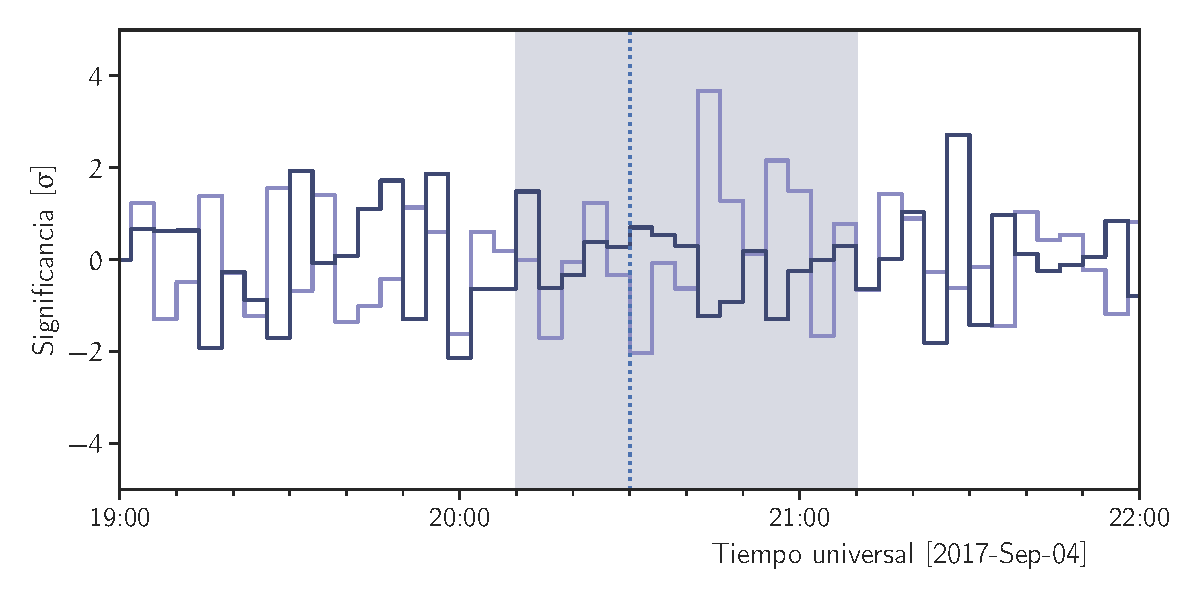
\includegraphics[width=\textwidth]{significance-170904.pdf}
        \caption{Significancia en función del tiempo para los grupos de hadrones (serie color violeta) y muones/electromagnética (serie color azul fuerte).}
        \label{fig:september-04-disc}
\end{figure}

Aunado a esto, la serie de hadrones tiene \num{4} excesos positivos posteriores al máximo, lo cual podría estar relacionados con neutrones de menor energía. Tomando en cuenta estos excesos la significancia está entre $5.1\sigma$ y $10.1\sigma$, dependiendo cuanto consideremos que dura la emisión. También existe la posibilidad que estos las dos señales significativas se presenten debido a dos instantes de aceleración diferentes, tomando en cuenta los dos máximos en emisión de rayos X duros. En este sentido un análisis más detallado del espectro registrado por FERMI y RHESSI puede dar pistas sobre el escenario en el que se aceleraron los neutrones.

\subsection{Posible observación de rayos $\gamma$ solares el 6 de Septiembre de 2017}

El \num{6} de Septiembre de \num{2017} el Sol produjo otra ráfaga tipo M\num{2.7} a las \DTMtime{15:45:00} UT, proveniente de la misma región activa que la explosión analizada previamente (aunque desplazada \SI{20}{\degree} al Oeste). La figura \ref{fig:september-06-flare} muestra una imagen de la atmósfera solar en la banda de \SI{13.1}{\nano\metre}.

\begin{figure}
        \centering
        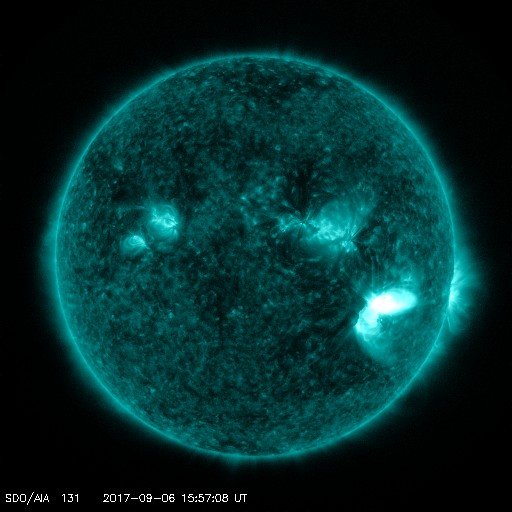
\includegraphics[width=0.7\textwidth]{sdo170906-1550-13}
        \caption{Image tomada por el satélite SDO durante la fulguración del $06/09/17$ en la banda de \SI{13.1}{\nano\metre}. Fuente: \url{https://www.spaceweatherlive.com/en.html}}
        \label{fig:september-06-flare}
\end{figure}

El satélite GOES registró el incremento en la banda de rayos X suaves, sin embargo ni FERMI ni RHESSI estuvieron en condiciones para observar este evento.

Aun con estas limitaciones, al revisar las condiciones para la detección de partículas solares, vemos que el SciCRT tenía buenas posibilidades de observarlas. Esto se puede corroborar mediante la figura \ref{fig:september-06-gammas}, en la cual se muestra que los mejores sitios para observar en el instante de la fulguración son Sierra Negra y Chacaltaya, Bolivia. El ángulo cenital solar es de \SI{45.1}{\degree} en el instante de la ráfaga, con una masa de aire de \SI{813}{\gram\per\square\cm} (masa efectiva de\SI{688}{\gram\per\square\cm}).

\begin{figure}
        \centering
        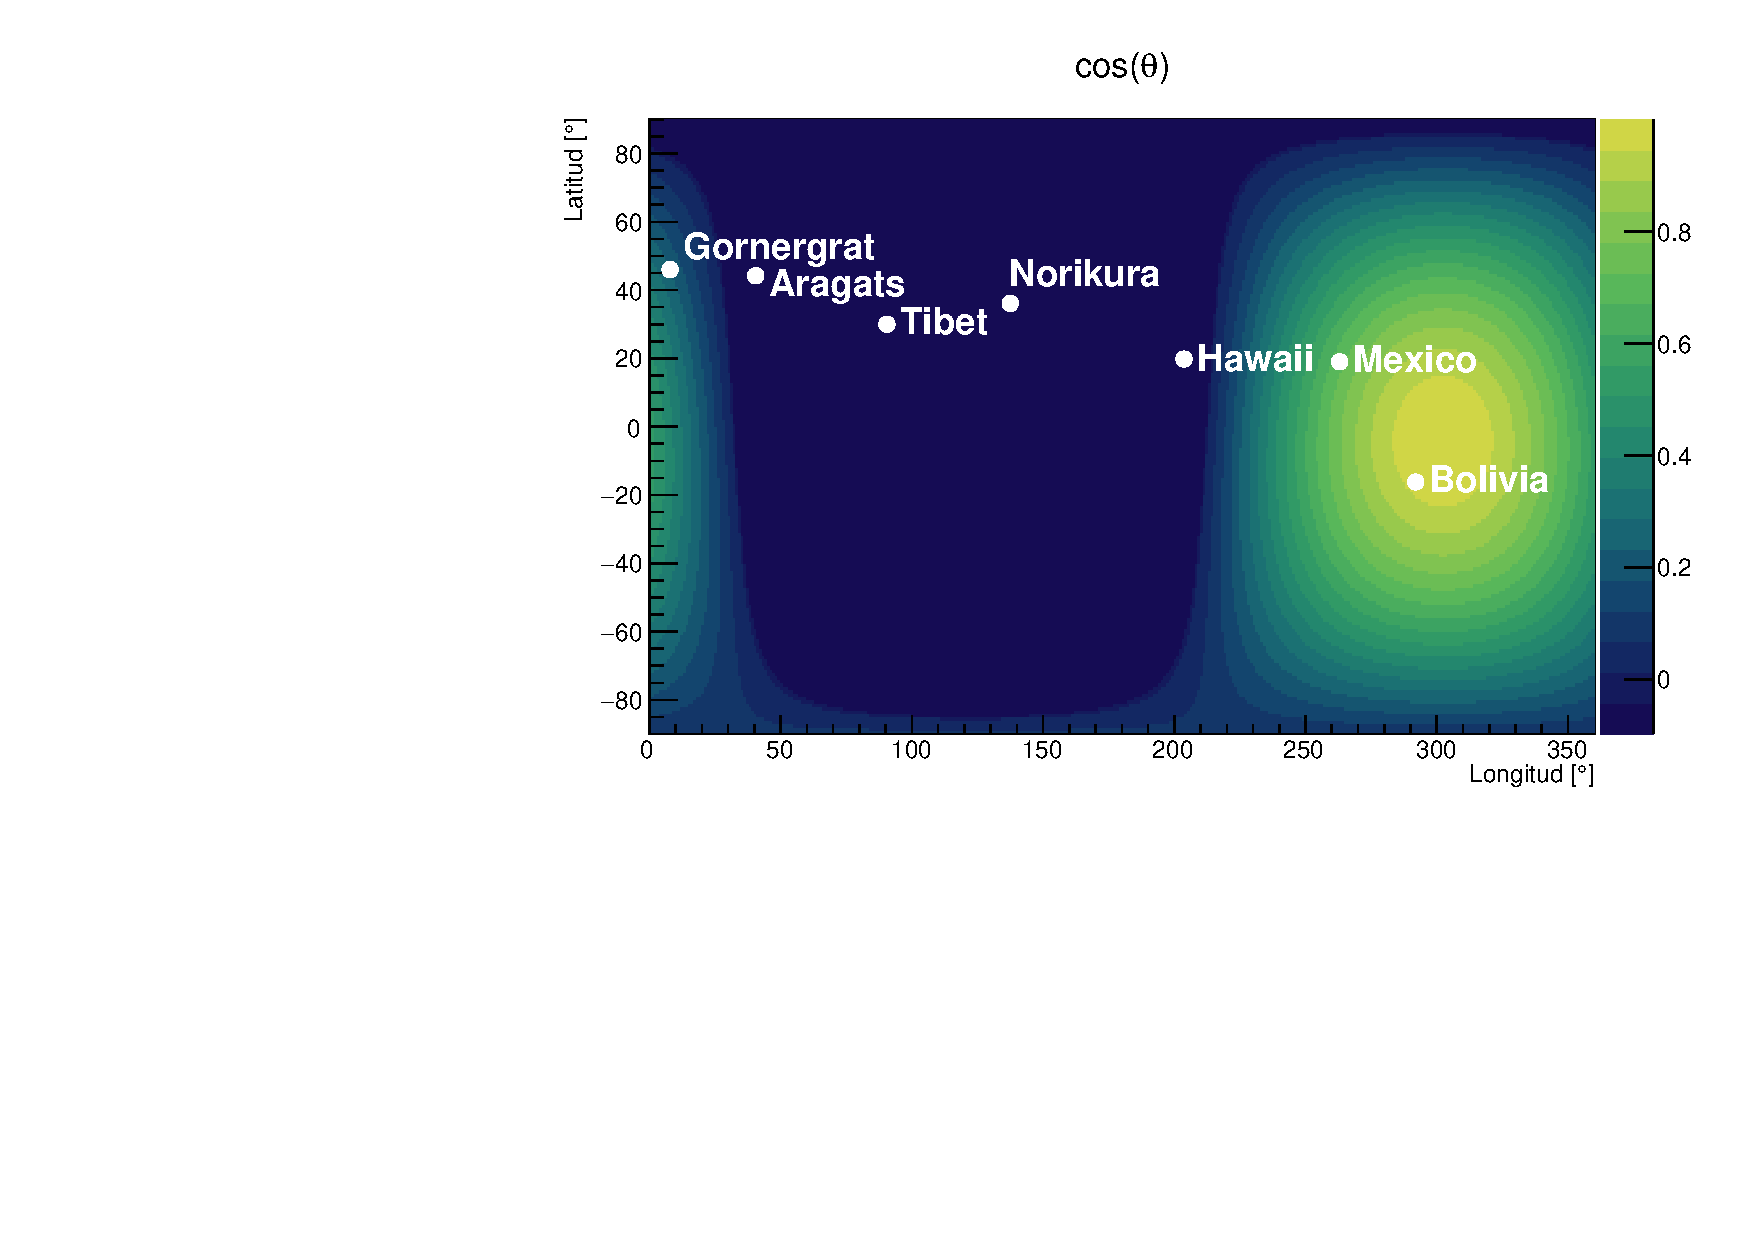
\includegraphics[width=0.8\textwidth]{cosz_170906.pdf}
        \caption{Coseno del ángulo cenital del Sol para el instante en que se registra la ráfaga. Los puntos muestran la localización geográfica de los TNS. La zona más clara indica un ángulo cenital del Sol cercano a cero.}
        \label{fig:september-06-zenith}
\end{figure}

La figura \ref{fig:september-06-neutrons} muestra la tasa de eventos registrada para el instante de la ráfaga, considerando la ventana de $t_{0}\pm\SI{1.5}{\hour}$. La linea azul representa el ajuste del polinomio de tercer grado, mientras que el área sombreada en la dirección horizontal es el intervalo de $\pm 3\sigma$. Para este evento en particular tenemos un exceso de $3.8\sigma$, seguido de \num{6} excesos positivos; resultando en una significancia de $8.9\sigma$ durante \SI{14}{\minute}.

\begin{figure}
        \centering
        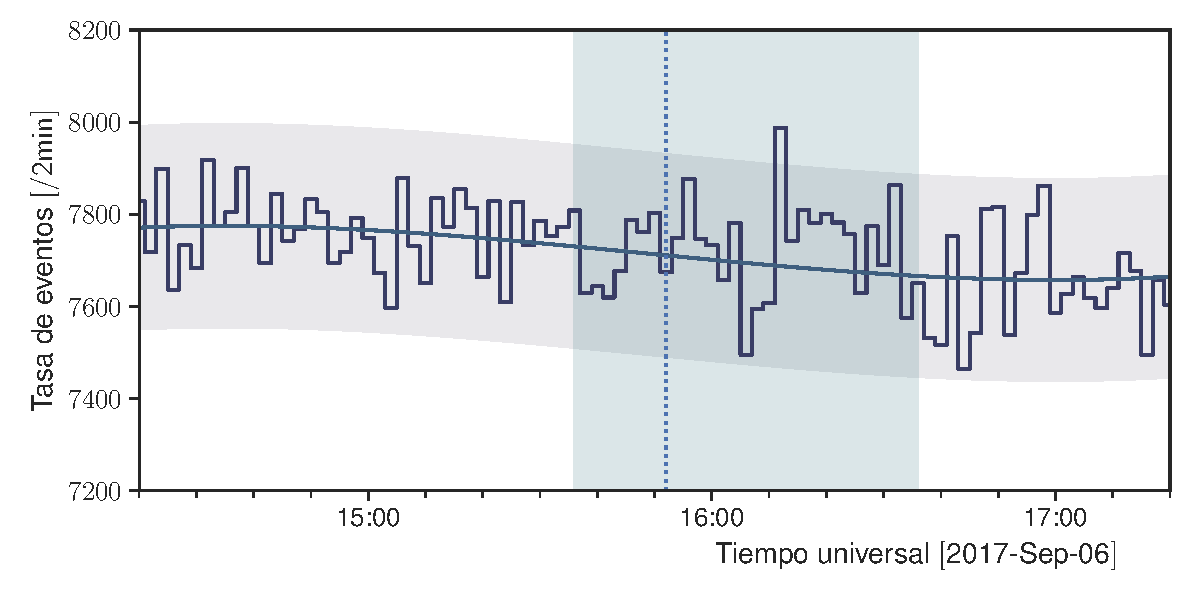
\includegraphics[width=\textwidth]{neutron-170906.pdf}
        \caption{Perfil temporal de eventos registrados por el SciCRT el $06/09/17$. El área sombreada representa el nivel de $3.0\sigma$.}
        \label{fig:september-06-neutrons}
\end{figure}

Por otro lado, aunque la señal es muy significativa para descartarla, sostener la hipótesis de que estas partículas son neutrones es difícil debido al retardo de \SI{20}{\minute} que existe entre $t_{0}$ y el exceso de $3.8\sigma$. De ser neutrones estas partículas, su energía cinética seria de \SI{100}{\mega\electronvolt} y los subsecuentes incrementos de menor energía; lo cual apuntaría a un espectro de emisión muy suave. Otra posibilidad de interpretar este resultado es que los iones primarios en la atmósfera solar no se hayan producido en el mismo instante que los electrones, llevando a este retraso. Ambos posibilidades pueden ser estudiadas analizando con detalle la distribución de energía depositada, lo cual se deja para un futuro estudio.

Otro posibilidad que surge de este resultado es que las partículas detectadas no sean neutrones. En este sentido el satélite GOES reporta un flujo de protones energéticos en la órbita terrestre, sin embargo esta hipótesis también resulta muy poco probable por dos circunstancias. La primera es que los protones monitoreados por GOES son de energías menores a \SI{1}{\giga\electronvolt}, lo que hace imposible que lleguen al sitio de Sierra Negra debido a la rigidez umbral del sitio ($\approx\SI{8.2}{\giga\electronvolt}$). Aunado a esto, no hay ningún exceso registrado asociado a estas partículas en la base de datos de monitores de neutrones (\url{https://www.nmdb.eu/nest/}).

Más aún, el incremento reportado por GOES inicia a las \DTMtime{12:02:00}, asociado a una fulguración muy intensa del tipo X\num{9.3}. En el caso de que un pequeño número de los protones producidos durante esta ráfaga tuviera la energía suficiente para entrar en la localidad de Sierra Negra, surge el problema de por qué se observan su detección a las \DTMtime{16:15:00}.

Otro escenario es el de la detección de rayos $\gamma$ solares. En este caso FERMI reporta una emisión de rayos $\gamma$ con energía $>\SI{100}{\mega\electronvolt}$, iniciando con la fulguración X\num{9.3} y manteniéndose durante más de \SI{13}{\hour} dos ordenes de magnitud arriba de la línea de base. Los datos de FERMI se muestran en la figura \ref{fig:september-06-gammas}, con la linea punteada indicando $t_{0}$ para la ráfaga M\num{2.6}. La linea negra solida representa el nivel de flujo de Sol quieto ($\approx\SI{4.5e-5}{\per\square\cm\per\second}$).

\begin{figure}
        \centering
        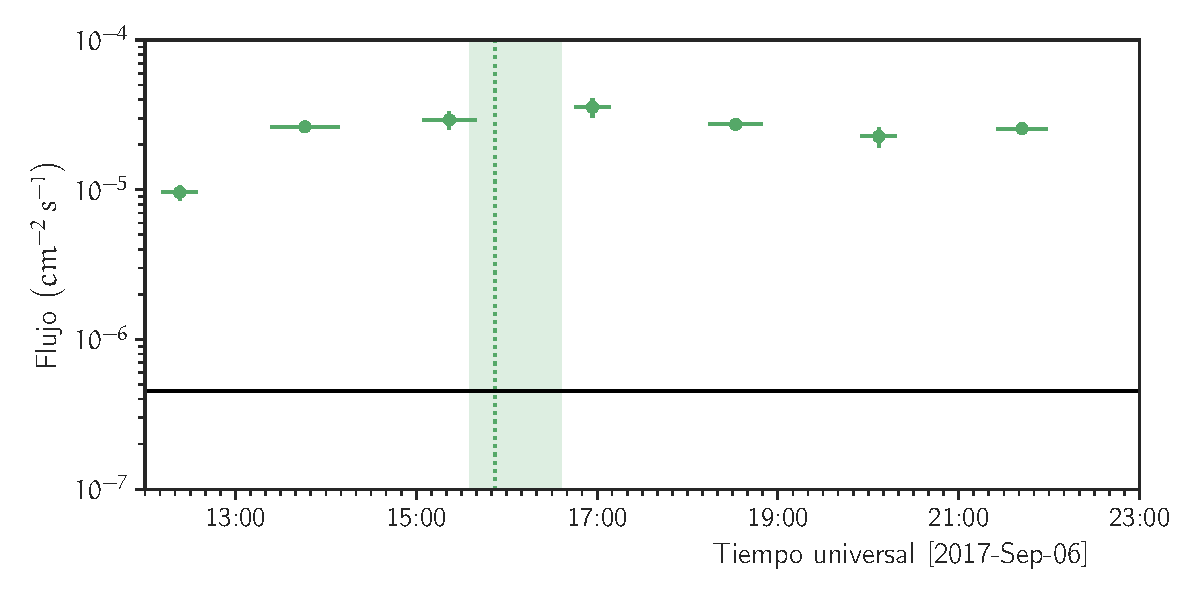
\includegraphics[width=\textwidth]{gammas-170906.pdf}
        \caption{Flujo de rayos $\gamma$ con energías $>\SI{100}{\mega\electronvolt}$ detectado por FERMI el $06/09/17$.}
        \label{fig:september-06-gammas}
\end{figure}

Para poder descartar las diferentes posibilidades, seguí una metodología similar a la hecha para el evento del \num{4} de Septiembre y apliqué el criterio de separación antes mencionado. De esta forma obtuve el resultado de la figura \ref{fig:september-06-disc}. Como se observa, para este evento el exceso se encuentra registrado en la serie de tiempo de la componente electromagnética/muones, con lo que en principio nos brinda pruebas de que las partículas detectadas son rayos $\gamma$.

\begin{figure}
        \centering
        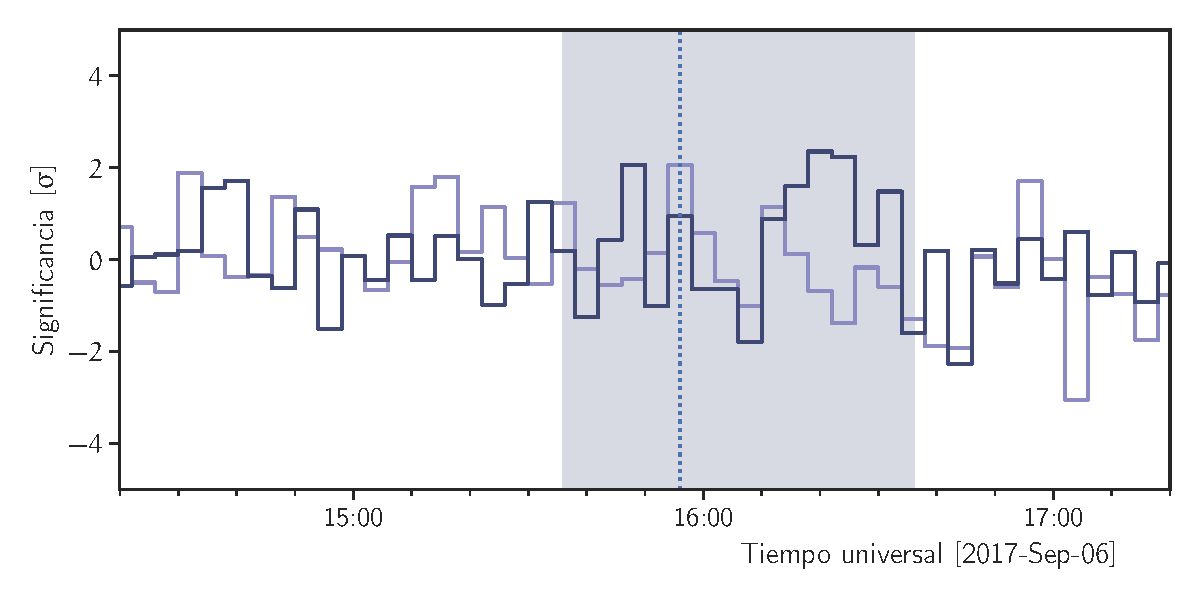
\includegraphics[width=\textwidth]{significance-170906.pdf}
        \caption{Significancia en función del tiempo para los grupos de hadrones (serie violeta) y muones/electromagnética (serie azul fuerte).}
        \label{fig:september-06-disc}
\end{figure}

Aun con este resultado, sustentar la hipótesis de la detección de rayos $\gamma$ es complicado, en primer lugar porque la atmósfera terrestre es opaca a este tipo de radiación. Por otra parte, esta hipótesis sufre del mismo problema que la detección de protones, debido a los intervalos de tiempo en que se registra. Con respecto a este ultimo punto, un argumento a favor es el presentando en \cite{muraki20}, en donde se reporta una detección de rayos $\gamma$ solares bajo circunstancias similares.
